\documentclass[11pt]{article}

\sepackage{graphicx}

\begin{document}
Elliott Capek \\

\begin{figure}[h!]
\centering
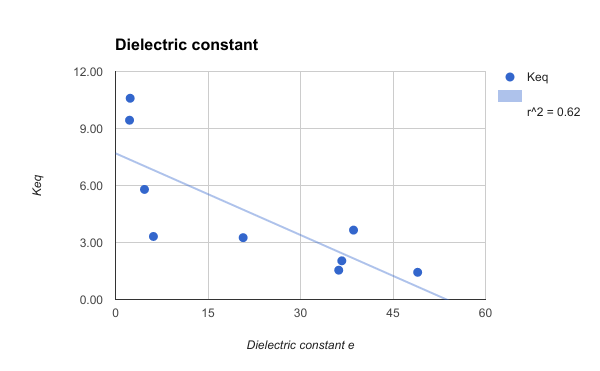
\includegraphics[width=0.75\textwidth]{image.png}
\caption{Data from timing threaded versus process programs. This is strange behavior. For this range of numbers, 100 million, adding more processes makes the situation worse once you have more than eight processes or one thread. This probably shows a problem in my implementation, although for reasons described below, this level of work might not actually benefit from more parallelization. The main thread calls new threads every time it gets a timeslice. However if the threads are completing in between main() timeslices, then more threads doesn't mean more speed..}
\end{figure}

\section{Design}
This project is broken up into two separate pieces: a threaded portion and a multi-process portion. Both processes share certain functions, which are implemented almost identically: a sieve function which takes an integer input and marks as composite all multiples of that integer and a function which calculates whether an input integer is happy.\\

The sieve function is simple. It just modifies an integer array (memory mapped or normal). The happy function is also simple. It applies the happy number algorithm repeatedly and after each iteration adds the next number to a dynamic array. Once the next number is 1, it returns a 1. If the next number is ever found in the dynamic array, that means the cycle is looping and the number will never be happy, so it returns a 0.\\

The threaded program will take as input the number of threads to use and the maximum number for its range. This will allow for a script to dynamically time its behavior. The program will use mutexes and conditional variables. TLPI has a very good example in its second Threads chapter on how to use conditional variables to launch several threads, then stop them all. The example uses a conditional variable sort of like a semaphore. Every time a thread is about to die, it locks the mutex, decrements a thread counter, changes its state to terminated, unlocks the mutex and dies. Meanwhile the main thread wait()s on the worker threads. This wait functions works so that the main thread has the death mutex at all times except when it is waiting. Thusly threads can only die when the main thread is waiting for them to die. After the wait stops blocking, the main thread checks its children for termination. I will need to keep these threads working after they terminate, so I will have the program at this point refresh each thread and call it anew. I will repeat this loop until the Sieve of Eratosthenes has gone through all the numbers, up to the square root of the max prime. After this is done I will use the exact same method to figure out which primes are happy, except I will do no thread refreshing and instead just evenly distribute the work among all threads. After this I will somehow write all the happy primes to a file.\\

The multiprocess program will basically work the same way. It will do all the same behavior and use the same functions, slightly modified. Instead of making a bunch of new threads, it will fork(). The child process will do the child function (sieving or finding happiness). These functions will end with an exit call. To sieve, the program will start with two, have a child sieve that number, find the next prime, sieve on that number, etc etc until the square root of the max prime has been sieved. The sieve will then be complete. To make sure no more than PROCESSES processes are running, I will first make PROCESSES processes. I will have a data structure to count the aliveness / deadness of each child. I will then use the waitpid() function almost exactly like the conditional wait function of the threaded application to wait for processes to die, then renew them. In this way I will keep sieving until the primes are all found. I will then evenly distribute the work of calculating happiness among the child processes, write to file and be done. \\


\section{Worklog}
\textbf{Friday July 31st 12:00pm-3:00pm} - Review TLPI book on topics: threads, mutexes, conditional variables, forking, shared memory, semaphores. Write design.\\
\textbf{Friday July 31st 3:30pm-5:00pm} - Wrote is happy function. Wrote dynamic array implementation for use in ishappy. Wrote single-thread Sieve of Eratosthenes implementation. \\
\textbf{Saturday August 1st 11:30pm-1:00pm} - Start on threaded implementation. Get application to successfully create threads and use mutexes on thread counter. Encountered weird bug where multiple threads would die when I expected only one to. Figured out it's because signaling a conditional variable doesn't immediately run the process waiting on it. Multiple threads would die and signal, then the waiting process would run. Fixed this bug by allowing for multiple thread deaths per wait.\\
\textbf{Saturday August 1st 1:30pm-5:00pm} - Debugged another weird bug which had a really easy solution. I found that threads were behaving weirdly and somehow having their states set from alive to terminated even though they hadn't even started running yet. After much searching, found it was because I didn't make sure all threads were dead before going on to the next operation. One thread would sometimes stay alive long enough to make it into the next set of threads and then terminate, causing weird behavior. \\
\textbf{Sunday August 2nd 11:00am-12:00pm} - Put finishing touches on threaded program. \\
\textbf{Sunday August 2nd 12:30pm-3:00pm} - Began implementing multi-process program. Did more research on how I wanted to have the processes interact with each other. Successfully got processes to sieve through a range by modifying threaded program.\\
\textbf{Sunday August 2nd 3:00pm-7:00pm} - Debugged minor issues, like shared memory not being truncated before use. Began implementing the ishappy functionality. \\
\textbf{Sunday August 2nd 7:00pm-9:00pm} - Finished the ishappy functionality. Began researching how to write output to a file. For some reason spent lots of time thinking about how to take an integer and convert it into a binary-representation string, then sprintf to a file. \\
\textbf{Monday August 3rd 11:00am-2:00pm} - Realized that write() was a much better solution than printing to a file. Implemented functionality to open happy primes file, truncate it, and write an unsigned int array to it. Spent a lot of time trying to figure out why my read() couldn't understand what I had just written to the file. Turned out I hadn't lseek()'d to the beginning of the file after I wrote, so of course I couldn't read what I had written. \\
\textbf{Sunday August 2nd 2:30pm-5:00pm} - Put finishing touches on programs, removed unnecessary pieces. \\
\textbf{Sunday August 2nd 5:00pm-7:00pm} - Moved code to server. Hit several problems. First, my programs couldn't be compiled initially because the heap arrays I was making were way too large (range from 0 to UINT MAX). Researched the icc flags to allow this behavior. Second, my programs kept getting killed the second they were executed. Internet says this is because the kernel thought they were too big at the time. Never fixed this bug. Found the key is to wait until not so many other procrastinating students are running their code. \\
\textbf{Sunday August 2nd 7:00pm-10:00pm} - Begin timing code and composing writeup. \\



\section{Challenges}
This was a challenging but very good assignment. I learned a lot about how multithreaded and multiprocess programs work. This was an assignment where I had to spend lots of time reading TLPI to figure out how I wanted to make my program. I was challenged with different implementations - to use semaphores or block on waitpid()s, or to use signals. Etc. \\

The hardest challenge was debugging a stochastic problem in my threaded program. It would show up maybe 1/3 of the time, but sometimes almost never, such that I thought it was gone. The problem was that I wasn't killing all my threads from a previous function (sieving through the primes), so when I tried to coordinate threads to figure out the happy primes of my sieve, some of the threads would die before I could use them. This screwed up the whole execution of the program, since I needed my thread-count variable to accurately reflect the number of threads alive and dead. It took a long time to figure out the source of the error, but I learned a lot. My takeaway from this is that programming slowly and diligently and making sure I think of all edge cases as I write a section of code is much better than quickly writing up a function and debugging it later. \\

\section{Questions}
\textbf{Point of assignment}: The point of this assignment is to have students become familiar with both threads and processes. This assignment is an introduction into parallel programming and sheds light on which approach (threads or processes) is appropriate to what situation. It also teaches how to have different processes communicate via signals, conditional variables, semaphores and mutexes. It also has students learn about how shared memory can be used to easily and quickly link program memory to disk memory.\\

\textbf{Correctness testing}: To test for correctness, I used the OEIS file for the first 10,000 happy primes. I had both my programs output data using the same formatting as the web database. I then did a diff between my outputted files and a downloaded copy of the database. The diff had no output, showing there was no difference between my file and the database. To test my file was being properly binary-dumped into a file, I read() that file and did a line-by-line comparison of the written and read arrays. \\

\textbf{What was learned}: My takeaway from this assignment is that threads are much easier to use than processes for parallel computing. When I was writing the programs I felt that threads were a much more elegant solution, since they already have shared memory implicitly (although I was very surprised by how easy to use shared memory was). Processes were slightly easier to use in that they just signaled when they were about to terminate and didn't need to use a mutex, whereas threads needed to use a mutex to signal with a conditional variable. This is a very minor difference, though. I also learned that shared memory is incredibly powerful, since it allows processes to essentially share data without having to coordinate at all. \\

\end{document}
